\documentclass[conference]{IEEEtran}
\usepackage[T1]{fontenc}
\usepackage[utf8]{inputenc}
\usepackage{cite}
\usepackage{graphicx}
\usepackage{booktabs}
\usepackage{tabularx}
\usepackage{array}
\usepackage{tikz}
\usetikzlibrary{arrows.meta,positioning}
\title{AgriPlus Mobile Decision Support for Coffee Leaf Health Screening and Farm Management}
\author{\IEEEauthorblockN{Akshay Kumar A}
\IEEEauthorblockA{Department of Master of Computer Applications\\
Nitte (Deemed to be University), NMAM Institute of Technology (NMAMIT)\\
Nitte, India\\akshayckm05@gmail.com}
\\[0.6ex]\textit{Faculty Mentor: Mamatha Balipa}\\
\IEEEauthorblockA{Department of MCA\\
Nitte (Deemed to be University), NMAM Institute of Technology (NMAMIT)\\
Nitte, India\\mamathabalipa@nitte.edu.in}}
\begin{document}
\maketitle
\begin{abstract}
Coffee growers often have to decide what to do with a leaf symptom before they can reach an advisor. AgriPlus is an Android prototype intended to support that first step: it accepts a leaf photo, requests a hosted classifier result, and places the scan alongside farm records and practical tools. The app is built with Kotlin and Jetpack Compose; Firebase provides sign-in and user-associated history. A local image check warns about brightness, contrast, and repeated selections, while the interface withholds predictions below a fixed score threshold. Inspection of the source shows that classification currently requires the remote service, even though TensorFlow Lite assets are bundled. The repository contains no labeled test set, model description, independent performance results, or grower evaluation. We therefore examine implemented behavior and deployment gaps rather than claim diagnostic accuracy, and outline the evidence needed for a field study.
\end{abstract}
\begin{IEEEkeywords}
coffee leaf screening, mobile decision support, plant disease recognition, Android, image quality, precision agriculture
\end{IEEEkeywords}


\section*{I INTRODUCTION}

For coffee farms, noticing a change on a leaf is often the beginning of a decision, not the decision itself. A grower may need to compare symptoms, check local conditions, record what was observed, and decide whether to seek expert help. Phone cameras offer a convenient way to collect an image, but the same symptom may look different across varieties, disease stages, lighting, viewing angle, and background. A mobile classifier can therefore assist screening only if users understand its uncertainty and can follow up on its output.

Image classifiers have performed well on benchmark collections, although benchmark performance alone says little about how a model will behave on a farmer's phone. On PlantVillage, Mohanty et al. reported 99.35\% on a held-out set; on images collected independently from online sources, the reported figure was 31.4\% [1]. This gap makes capture conditions and test-set design central to deployment claims. Coffee datasets provide more relevant evaluation material: RoCoLe includes field smartphone photographs and expert-reviewed categories for healthy leaves, mites, and rust severity [2]; JMuBEN and JMuBEN2 add a larger Arabica collection spanning five classes [3]. Neither dataset validates the separate service used by AgriPlus.

We examine AgriPlus as a software artifact that connects a photo-based screening flow with farm-management functions. A selected image passes through a basic local check and is sent to a hosted service; the returned class is mapped to explanatory text and can be saved in the user's history. Other screens cover weather context, plantations, treatment information, reminders, consultation, analytics, and comparison of scans. The sections below describe what is present in the source and separate those observations from results that the project has not measured.

This study contributes a traceable description of the app's image-to-service path and its surrounding data flow; an inspection of consequential implementation choices, including the fixed 0.60 cutoff, advisory-only image warnings, Base64 image storage, and a credential packaged with the client; and a staged evaluation plan covering model behavior, field capture, software reliability, and user understanding. It introduces neither a new classifier nor a new dataset, and reports no diagnostic benchmark.

\section*{II RELATED WORK}

\subsection*{A Plant Disease Recognition and Domain Shift}

Results from curated photographs can overstate readiness for outdoor use. The difference between the two test settings in [1] is a practical warning: a random split may retain visual cues shared by images from the same source, while images from another collection expose changes in background and acquisition. Evaluation for farm use should therefore group data by plant, site, or capture session when repeated images are present. Ferentinos' survey of convolutional plant-disease models provides a wider basis for automated diagnosis research [6]. For an application, headline accuracy should be supplemented with calibration, class-specific errors, rejection rates, and tests on naturally captured images.

\subsection*{B Coffee Datasets and Mobile Systems}

The available coffee image collections differ in crop type, sampling, labels, and annotation. RoCoLe contains 1,560 phone photographs from 390 Robusta plants. Its six labels include healthy leaves, mites, and four rust levels, with expert-reviewed reference labels [2]. The JMuBEN collections contain 58,555 Arabica images labeled for Phoma, Cercospora, rust, miner, or healthy leaves, collected in Kenya with pathology input [3]. For natural backgrounds, Tassis et al. pair leaf segmentation with disease and pest recognition on in-field smartphone images [4]. Hitimana et al. describe a coffee reporting app that combines a deep-learning workflow with location-linked reporting and farmer information tools [5].

AgriPlus is adjacent to these systems in its mobile workflow, but the available artifact supports a different kind of report. Its Android code shows how the client calls an inference endpoint; it does not identify the service's training images, network design, per-class results, or model documentation. A numerical comparison with the studies above would therefore be unsupported. The focus here is the client implementation, the farm features around screening, and the limits that remain visible in the repository.

Taken together, the prior work supports three distinct evaluation settings: controlled data for model development, field-collected photographs for testing capture variability, and mobile workflows that retain enough context for follow-up. These settings answer different questions and should not be conflated. AgriPlus performs image preparation on the handset and requests a remote classification, but its repository does not include a reproducible training process or a validated image set for that service. Our conclusions are limited accordingly.

\section*{III SYSTEM DESIGN AND METHODS}

\subsection*{A Artifact-Based Study}

We conducted a source-based implementation review. We followed the Android navigation graph into the scan screen, traced image preparation and the API request, examined result parsing and history writes, and inspected the data managers used by the other feature areas. A debug build was installed and launched on one handset to confirm that the package starts. This narrow check establishes neither end-to-end correctness nor speed, usability, or agronomic validity.

We report only behavior that can be traced to the code or the single launch check. The project files do not provide coffee-leaf labels, training scripts, a specification for the hosted classifier, a frozen response set, or records from a field trial. Because those materials are absent, this paper gives no estimate of accuracy, precision, recall, F1, inference time, or farmer acceptance.

\section*{B Application Workflow}

AgriPlus uses a Kotlin single-activity client with Compose screens and Navigation Compose. Google sign-in establishes a Firebase Authentication session; history entries are written beneath that account's UID in Realtime Database. A scan begins when the user supplies a camera image or chooses one from the gallery. The client runs local quality heuristics, encodes the image as JPEG, and sends it to the hosted classifier.

\begin{figure}[!t]
\centering
\resizebox{\columnwidth}{!}{%
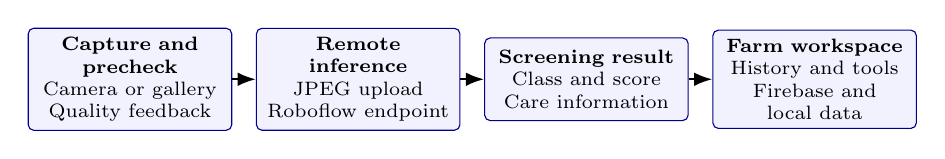
\begin{tikzpicture}[node distance=3mm, >=Latex,
  box/.style={draw=blue!55!black, rounded corners=2pt, fill=blue!5,
    text width=2.35cm, minimum height=1.05cm, align=center, font=\scriptsize}]
\node[box] (a) {\textbf{Capture and precheck}\\Camera or gallery\\Quality feedback};
\node[box, right=of a] (b) {\textbf{Remote inference}\\JPEG upload\\Roboflow endpoint};
\node[box, right=of b] (c) {\textbf{Screening result}\\Class and score\\Care information};
\node[box, right=of c] (d) {\textbf{Farm workspace}\\History and tools\\Firebase and local data};
\draw[->, thick] (a) -- (b); \draw[->, thick] (b) -- (c); \draw[->, thick] (c) -- (d);
\end{tikzpicture}%
}
\caption{Implemented AgriPlus workflow; local farm tools and weather context surround the network-dependent image-inference path.}
\label{fig:architecture}
\end{figure}

\subsection*{C Image Intake and Quality Feedback}

The checker first resizes a bitmap to 64 by 64 pixels. It uses mean brightness to flag very dark inputs (below 42) and very bright inputs (above 228) on an 8-bit scale. It also averages neighboring-pixel luminance differences and warns when the value is under 5.2, and compares a 64-bit luminance hash with recent choices to detect repeats during the current screen session. These quick rules have not been validated against expert image ratings. The UI shows the warning, but the returned validity value does not block submission. The preview camera path also supplies a reduced-resolution image.

\subsection*{D Remote Prediction and Result Mapping}

For the request, the selected bitmap is JPEG-compressed and posted through OkHttp to a Roboflow serverless endpoint. The client reads the first prediction's label and score from the JSON response. The screen declines to show scores below 0.60 and asks for another image. For a recognized label, a local repository supplies a disease name and fixed text about causes, symptoms, and treatment; other labels receive a generic explanation. The 0.60 value is embedded in the client. No calibration study shows that it corresponds to a particular probability of correctness.

The APK also contains a TensorFlow Lite model, a label file, and a `LeafClassifier` implementation. However, the active `HomeScreen` scan path calls the network API rather than this local classifier. The bundled assets therefore do not make the present scan function available offline; a successful prediction currently depends on connectivity and the remote service.

\section*{IV IMPLEMENTATION}

For each visible workflow, we traced its corresponding implementation where the repository allowed it: navigation into a screen, image handling, request construction, response fields, and persistence. We also checked what data sources and fallback paths the feature modules use. This is an implementation review, not a complete audit of all runtime paths or backend configuration. In particular, it cannot establish how remote services are configured beyond what the client code exposes.

The codebase brings together Compose screens, screen-level state, and helper classes. It is organized as a working prototype rather than a strict ViewModel-centered architecture: the home screen coordinates much of the scan request, response parsing, and result display, while managers cover selected storage and external requests. Table I records the feature groups visible in the source and the main caveat attached to each.

\begin{table}[!t]
\caption{Implemented feature groups and current boundaries}
\label{tab:features}
\centering
\scriptsize
\begin{tabularx}{\columnwidth}{>{\raggedright\arraybackslash}p{.19\columnwidth}>{\raggedright\arraybackslash}X>{\raggedright\arraybackslash}X}
\toprule
\textbf{Feature} & \textbf{Implementation} & \textbf{Boundary} \\
\midrule
Leaf screening & Camera/gallery; local warnings; remote label and score & No disclosed model card or measured accuracy \\
History & UID-scoped Firebase records; JPEG stored as Base64 & Payload size and retention require review \\
Farm tools & Plantations, reminders, treatment notes, analytics & Local preferences and cloud sync coexist \\
Weather & Open-Meteo forecast and rule-based coffee advisory & Fallback weather is synthetic, not live \\
Consultation & Keyword/category rules generate preliminary text & No human agronomist response is implemented \\
\bottomrule
\end{tabularx}
\end{table}

\subsection*{A Farm Management and Weather Modules}

Plantation profiles and blocks are kept locally and synchronized to the signed-in user's Firebase area. Reminders combine local preferences, Firebase records, and Android AlarmManager scheduling. Treatment entries and saved notes are available from a local guide. Weather and geocoding use Open-Meteo; when a request fails, the repository supplies preset values so the screen can still render. Those values are simulated fallbacks and should never be presented as a live forecast.

Consultation messages are generated by local keyword and category rules, then saved locally and remotely. Although the code marks the response with wording that suggests an extension officer has replied, the text is automated and no person reviews it. The interface should state this plainly and offer a route to an actual advisor before release to growers.

\subsection*{B Data Handling and Security}

Each history item stores the predicted label, score, timestamp, and JPEG encoded as Base64 beneath the user's UID. UID-specific paths organize records, but they do not demonstrate that the Firebase rules prevent unauthorized access. The inspected files do not establish how consent, image retention, deletion across services, or the inference provider's handling of uploads are configured. We also found the inference credential in client-side source. Since packaged credentials can be recovered from an app, this value should be rotated and replaced with a server-mediated request or a suitably restricted credential before a public release.

\subsection*{C Interaction, Accessibility and Failure States}

Users interpret more than the predicted class: they see the capture prompt, wait for a result, and decide what the score and explanation mean. The score is not known to be calibrated, so it should not be shown as the chance that the label is correct. The screen should describe the result as an initial screening aid, keep the analyzed image visible, and make it easy to retake an unclear photo or contact an expert. This is important because different leaf problems can look alike and field photos rarely match curated examples exactly.

The source review did not measure accessibility. Before wider use, the app should be checked for readable contrast in sunlight, scalable text, useful focus order, translated wording, and touch targets that work on common low-cost phones. Status must remain understandable without color alone, so warnings and uncertain results should also use clear labels and icons.

Important interruptions include denied camera permission, missing gallery access, lost connectivity, a slow or unavailable endpoint, an invalid response, or a failed history write after a prediction appears. Users should be able to retry and should be told whether the scan was saved. A failed upload must not look like a completed screening, and old weather values must not look current. Defining observable screen states—from image selection and upload through a result, a low-score rejection, or a recoverable error—would make these cases easier to check consistently.

\subsection*{D Data Lifecycle and Separation of Concerns}

The current record bundles result details with the image, although these data need not share a retention policy. A future data design should state separately whether the photo is uploaded for inference, kept in history, and stored by a provider, and for how long. Users should be able to remove stored scans, including image copies retained by services under the app's control. We could not verify the applicable access rules, consent text, retention period, or deletion process from the files reviewed, so this paper makes no claim about regulatory compliance.

The scan screen currently handles several responsibilities together: acquiring the image, starting the request, decoding the response, updating the screen, mapping the label, and saving the record. Moving service calls and response checks behind a typed repository would make the network path easier to replace and would give retries one clear owner. The response should also be checked for a known label and a finite score in the expected range before display. With those boundaries in place, a validated on-device classifier could later feed the same result view and history schema.

\section*{V ARTIFACT-BASED FINDINGS}

Source inspection confirms that the main scan path is connected: a person selects a leaf photo, sees local quality feedback, sends the image to the hosted service, and may receive mapped explanatory text and a saved history entry. The app also contains screens for weather, plantation data, treatment notes, reminders, consultation, analytics, and comparing scans. We built and launched a debug package on one handset. These are implementation observations, not classifier results.

The fixed score cutoff provides a rejection path, but there is no evidence that 0.60 is an appropriate boundary for any particular disease. Likewise, the image checker can alert a user but does not prevent an image from reaching the classifier. The farm tools could make a scan more useful by supporting follow-up, yet they also make it important to distinguish current weather from preset fallback data and human guidance from automated text.

The evidence supports an integrated mobile workflow, not a validated diagnostic tool. Because the Android repository does not identify a fixed model build or its training data, the same label cannot yet be tied to a reproducible classifier version. The app's local explanation map can also fall out of sync if the endpoint changes its class names. A versioned response format and model identifier saved with each scan would make later review and comparison more meaningful.

\section*{VI DISCUSSION}

An isolated prediction screen offers little support for what a grower does after seeing a label. AgriPlus connects scans with records, reminders, treatment information, and weather context, supporting follow-up across visits. This is similar in aim to the reporting functions described by Hitimana et al. [5], but AgriPlus relies on a remote classifier and its repository contains no training or field-evaluation record.

Two questions remain open: whether the classifier is dependable on coffee farms and whether the app helps growers complete a useful task. Smooth navigation cannot resolve domain shift, overlapping symptoms, or an unjustified score cutoff. A benchmark cannot show whether growers can take a usable picture, interpret uncertainty, and act safely. Future work should measure software, model, service, and user outcomes separately while examining how they interact.

Mislabeling an affected leaf as healthy could postpone inspection; labeling a healthy leaf as diseased could prompt unnecessary effort or expense. The practical effect depends on the condition and suggested response. One overall accuracy figure would conceal these distinctions. Evaluation should report class-wise sensitivity and precision, then test whether scores can route uncertain cases toward another photo or qualified advice. The app can suggest a next step without presenting its output as a final diagnosis.

If the hosted classifier changes over time, the team needs a way to identify shifts in its behavior. Camera changes, preprocessing, retraining, or a revised label set can alter outputs. Recording app and model identifiers with each release would make results traceable; a governed audit set could help detect changes in class frequencies or low-score rates. Any image collection for monitoring needs a stated purpose and safeguards.

The weather feature applies rules to weather inputs; it is not a trained disease-forecast model. Present it as contextual guidance with its source and update time. Treatment entries are static and consultation replies are automated. Coffee specialists should review this material against current local recommendations and track revisions. Clear labels help prevent fluent generated text from being mistaken for an expert assessment.

\section*{VII LIMITATIONS AND FIELD VALIDATION PLAN}

Several missing artifacts constrain this review: we could not inspect a labeled training and test corpus, a model card, or observations from farm users, and the service behind the API may change without an app release. Image thresholds have not been compared with expert ratings or classifier errors. Our handset check confirmed startup only; it did not establish scan reliability, security rules, reminder delivery, user comprehension, or diagnostic correctness.

The next study should use a fixed, identified model and expert-labeled coffee images from multiple farms, varieties, seasons, phones, and lighting conditions. Separate training and evaluation data by plant and farm to avoid near-duplicate leakage. Report class-specific sensitivity, precision, and F1, as well as macro-averaged results, confusion matrices, score calibration, and the share of photos rejected at 0.60. Reserve an external farm set for final evaluation after model selection.

Annotators should record disease category and, where possible, severity; qualified plant-health reviewers should resolve disagreements. Include healthy leaves and visually similar conditions as well as clear disease examples. Retain study metadata such as farm, variety, date, device, lighting, and capture procedure so performance can be examined across settings. Before examining the locked set, specify inclusion rules, class mapping, threshold selection, and primary measures.

Software evaluation should measure how often the image check rejects usable photos or accepts poor ones, request times at typical and slow percentiles, upload volume, network recovery, and consistency across supported phones. In a formative study, observe growers and extension staff photographing leaves, interpreting uncertainty, retrieving earlier scans, and completing follow-up tasks. Obtain appropriate review and consent. A security review should inspect database rules, replace the client credential, document remote image handling, define retention and deletion, label fallback weather, and correct the suggestion that an officer authored automated replies.

The user study should examine comprehension as well as task completion. Ask participants to explain a class label and score, describe what they would do next, and say when they would seek a second opinion. Use the responses to revise plain-language explanations and escalation steps, with local terminology reviewed by extension staff. Weather and treatment screens should show source and freshness; chemical guidance should point to current locally approved material.

Set acceptance criteria before collecting results. For the classifier, stakeholders could define minimum sensitivity by class on external farms, a maximum calibration error, and an acceptable abstention rate. For the app, criteria could cover completing capture and history tasks during intermittent service, a response-time target, and verified removal of a saved image. Agronomy and product teams should agree on these limits before testing rather than tune them after seeing outcomes.

Introduce the system in stages: begin with a technical pilot using synthetic or consented examples, then have extension professionals review outputs in a supervised trial. Only after reviewing that evidence should a limited grower study begin, with clear screening language and a way to report problems. If external testing reveals serious class errors or unreliable scores, narrow the supported categories, revise the rejection policy, or suspend automated suggestions while keeping recordkeeping available.

The capture protocol should tell participants how many leaves to photograph, which surface to show, and how far away to hold the phone. Include examples for framing, glare, and shadow. Test the instructions with growers using different phones and camera experience. Compare quality warnings with expert ratings and classifier outcomes rather than assuming the current thresholds suit every device. Revise the guidance if it rejects useful images or accepts photos that repeatedly lead to errors.

Record whether users can decline to upload a photo, cancel a request in progress, and recover if a result cannot be saved. An offline state could retain access to non-diagnostic farm records while clearly disabling classification; it must not imply that an old prediction is current. These observations will show whether network-dependent screening is practical in the intended areas or whether a separately tested on-device classifier is needed.

\section*{VIII CONCLUSION}

We reviewed AgriPlus, an Android prototype linking coffee-leaf photo screening with farm records and related tools. Its source connects camera or gallery input, local image warnings, hosted inference, score-based result display, local text for disease labels, and Firebase history with weather, plantation, treatment, reminder, analytics, and consultation screens. The active scan requires the hosted service; the packaged TensorFlow Lite model is unused by that path; image checks do not block submission; and the repository provides no independent diagnostic or field-usability measurements.

The evidence supports feasibility of connecting these software components, not reliable coffee-disease diagnosis. Validation requires expert-labeled tests across farms, calibrated scores, a secured server-side credential, transparent advice sources, and grower-centered evaluation of the workflow.

\section*{REFERENCES}

[1] S. P. Mohanty, D. P. Hughes, and M. Salathé, ``Using deep learning for image-based plant disease detection,'' Frontiers in Plant Science, vol. 7, Art. no. 1419, 2016, doi: 10.3389/fpls.2016.01419.

[2] J. Parraga-Alava, K. Cusme, A. Loor, and E. Santander, ``RoCoLe: A robusta coffee leaf images dataset for evaluation of machine learning based methods in plant diseases recognition,'' Data in Brief, vol. 25, Art. no. 104414, 2019, doi: 10.1016/j.dib.2019.104414.

[3] J. Jepkoech, D. M. Mugo, B. K. Kenduiywo, and E. C. Too, ``Arabica coffee leaf images dataset for coffee leaf disease detection and classification,'' Data in Brief, vol. 36, Art. no. 107142, 2021, doi: 10.1016/j.dib.2021.107142.

[4] L. M. Tassis, J. E. T. de Souza, and R. A. Krohling, ``A deep learning approach combining instance and semantic segmentation to identify diseases and pests of coffee leaves from in-field images,'' Computers and Electronics in Agriculture, vol. 186, Art. no. 106191, 2021, doi: 10.1016/j.compag.2021.106191.

[5] E. Hitimana et al., ``Revolutionizing coffee farming: A mobile app with GPS-enabled reporting for rapid and accurate on-site detection of coffee leaf diseases using integrated deep learning,'' Software, vol. 3, no. 2, pp. 146--168, 2024, doi: 10.3390/software3020007.

[6] K. P. Ferentinos, ``Deep learning models for plant disease detection and diagnosis,'' Computers and Electronics in Agriculture, vol. 145, pp. 311--318, 2018, doi: 10.1016/j.compag.2018.01.009.
\end{document}
